\chapterimage{Week5Ponds.jpg} % Chapter heading image

\chapter{Stabilzation Ponds}
% Chapter heading image

\begin{itemize}
\item Stabilization ponds and lagoons are bodies of water which treat wastewater using mainly natural processes including sunlight, algae and microorganisms for treating wastewater\\
\item While ponds are shallow and man-made, lagoons are bodies of water confined within natural boundaries.\\
\end{itemize}


\section{Advantages of ponds}\index{Advantages of ponds}	

\begin{itemize}	
\item Cheap to build and operate
\item Low maintenance and electrical costs
\item Do not require highly trained operational personnel
\item Provide treatment that can be equal to some secondary treatment processes and have fewer sludge handling issues.\\
\end{itemize}


\section{Disadvantages of ponds}\index{Disadvantages of ponds}	
\begin{itemize}	
\item Land intensive
\item Effluent quality varies with seasonal temperature changes
\item Suspended solids levels that can create regulatory problems.
\item System upsets almost always result in odor problems and recovery times may be weeks or months.
\item Not appropriate for colder climates
\end{itemize} 

\section{Types of Ponds}\index{Types of Ponds}	

\subsection{Anaerobic Ponds}\index{Anaerobic Ponds}	

\subsubsection{Anaerobic Ponds}\index{Anaerobic Ponds}	

\begin{itemize}	
\item Typically for treating raw sewage
\item These are deep - 10-14 feet treatment ponds which rely primarily on anaerobic bacteria to break down the organic waste.
\item Designed for BOD removal.
\item High strength wastewater may be treated.
\item Organic matter is broken down releasing releasing methane, carbon dioxide and odorous gases including hydrogen sulfide. 
\item Most of the decomposition is accomplished by acid forming bacteria. 
\item The pH in these lagoons is usually below 6.5. 
\item They are total retention and do not have an effluent discharge. 
\item The anaerobic pond must be de-sludged approximately once every 2 to 5 years
\item Organic loading of 200-1000 lbs. $BOD_5$ per acre per day
\end{itemize}

\subsection{Facultative Ponds}\index{Facultative Ponds}	

\begin{itemize}
\item The depth of facultative ponds is about 4-7 feet which is in-between the depths of anaerobic ponds (10-14 feet) and aerobic ponds 3 feet)
\item The uper layer of facultative pond is aerobic, and bottom layer is mostly anaerobic.
\item Facultative bacteria are responsible for most of the treatment that occurs in these ponds.  Facultative bacteria are bacteria which can live under both aerobic and anaerobic conditions.
\item The algae that grow in the pond are critical to the successful stabilization of the organic load. 
\item The algae will take in carbon dioxide ($CO_2$) and, through photosynthesis, use it to create sugars and release dissolved oxygen ($O_2$) that is used by the aerobic bacteria. Facultative lagoon levels should always maintain at least 4 feet of water in the pond.
\item Typically for secondary treatment - BOD removal
\item 15-50 lbs $BOD_5$ per acre per day.
\item Unused CO$_2$ will react with water to form carbonic acid - which would reduce the pH unless consumed
\item Sludge removal need is rare.  Sludge can be removed by using a raft-mounted sludge pump or by draining and dewatering the pond and removing the sludge with a front-end loader.
\end{itemize} 

				\begin{sidewaysfigure}
\begin{center}
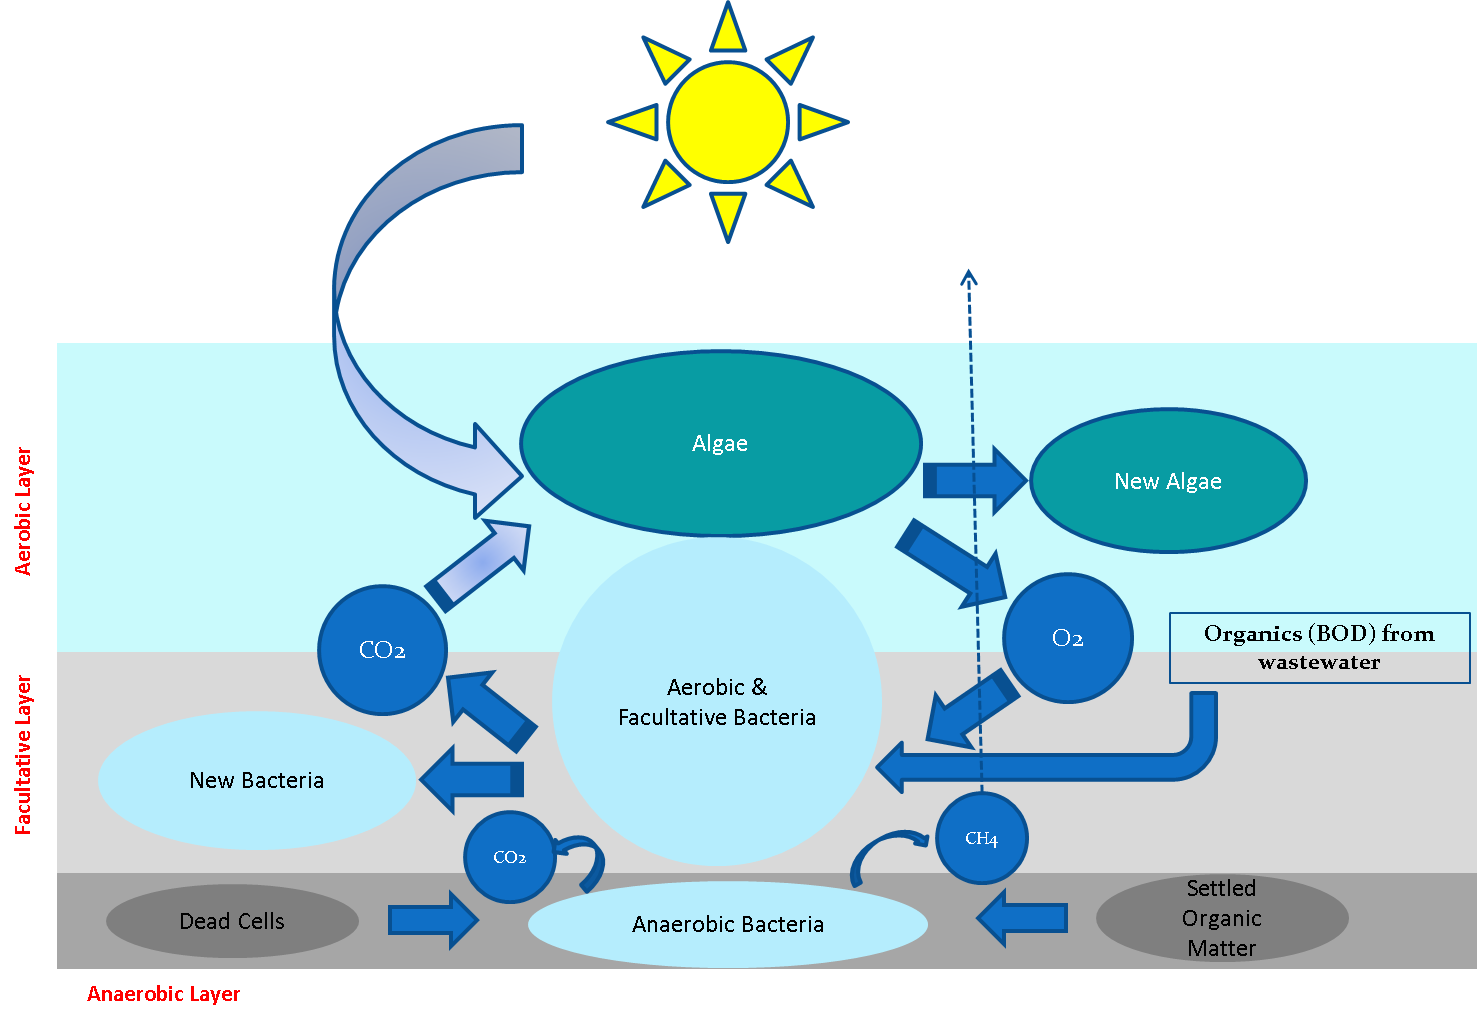
\includegraphics[scale=0.8]{StabilizationPond}\\
Facultative pond schematic
\end{center}
				\end{sidewaysfigure}
				
\subsection{Aerobic Stabilization Ponds}\index{Aerobic Stabilization Ponds}
	
Aerobic stabilization ponds are also known as: \hl{maturation}, \hl{polishing} or \hl{finishing} Pond
\begin{itemize}
\item Contain disssolved oxygen throughout entire depth of the pond.
\item Treatment is accomplished through the stabilization of organic wastes by aerobic bacteria and algae.
\item Typically for tertiary treatment
\item Designed for pathogen removal
\item Shallow - only about 3 feet deep. 
\item They are most often the final cells in a multi-staged pond system
\item They are also used as polishing ponds for tertiary treatment of trickling filter plant effluent.
\item Usually the effluent is directed into a second pond where the sludge can settle 
\item Their shallow depth allows sunlight to penetrate to the bottom of the pond to encourage algae growth and aerobic conditions throughout the pond 
\item The low solids loading found in these tertiary treatment applications means that these ponds normally have no sludge zone
\item These ponds may be mechanically aerated 
\item Aerobic polishing ponds are designed for 15-20 pounds BOD/acre/day
\item Aerobic ponds are typically designed for pathogen removal
\item Aerobic lagoon levels should always maintain at least 18 inches of water in the pond
\end{itemize}



\section{Ponds Operations and Maintenance}\index{Ponds Operations and Maintenance}

\begin{itemize}
\item Ponds and lagoons are designed as continuous discharge, controlled discharge, or no discharge.
\begin{itemize}
\item In controlled discharge ponds the wastewater is held for long periods of time before discharging. 

\item No-discharge ponds the inflow rate needs to be equal or exceed the rates of evaporation and/or percolation. 
\end{itemize}
\item Short-circuiting in a pond may be caused by poor design of inlet and outlet piping arrangements or by uncontrolled growth of water weeds.
\item Stagnant water will breed mosquitoes and can result in anaerobic conditions developing that can cause odor issues 
\item Dikes need to be maintained
\item Aquatic plants and weeds must be removed from the water. 
\item Reeds will create stagnant areas along the edge of the pond and need to be removed
\item To start a new pond, two feet of water is typically added prior to fresh starting wastewater feed. 
\item Sodium nitrate can be used to help recover from an odor-causing upset. The nitrates ($NO_3$) will provide a source of chemically bound oxygen for the bacteria to use instead of dissolved oxygen.
\item Scum control may be required
\end{itemize}





\newpage
\section*{Chapter Assessment}
\begin{tcolorbox}[breakable, enhanced,
colframe=blue!25,
colback=blue!10,
coltitle=blue!20!black,  
title= Chapter Assessment]

\begin{enumerate}

\item  Organic loading to a stabilization pond is always calculated by knowing the pounds of BOD applied per 1.000 cubic feet of pond volume per day.\\


a. True \\

b. False \\


\item  An abundance of aquatic plant growth in and around the edge of a facultative pond provides more surface area for biologic activity and increases treatment capacity.\\


a. True \\

b. False \\


\item  Facultative ponds are anaerobic on the bottom and aerobic near the surface.\\


a. True \\

b. False \\


\item  The best time of the year to initiate operation of a new facultative pond is during the coldest months of the year.\\


a. True \\

b. False \\


\item  Ponds that contain an aerobic top layer and an anaerobic bottom layer are called facultative ponds.\\


a. True \\

b. False \\


\item  One short-term corrective measure for an overloaded facultative pond might be to add:\\


a. copper sulfate . \\

b. sodium sulfide. \\

c. ammonium sulfide . \\

d. sodium nitrate. \\

e. potassium chloride. \\


\item  Photosynthesis is an essential part of the biological activity associated with:\\


a. Activated sludge \\

b. Trickling filters \\

c. Oxidation ditches \\

d. Aerobic digesters \\

e. Sewage lagoons \\


\item  During the process of algal photosynthesis:\\


a. Chlorophyll converts sunlight into energy for growth. \\

b. Algae produces oxygen \\

c. Algae converts CO2, NH3, and PO4, into additional algae cells \\

d. All of the above \\


\item  pH of the facultative pond will be the highest\\


a. during daytime when the consumption of CO2 is the highest \\

b. during daytime when the consumption of CO2 is the lowest \\

c. during nighttime when the production of CO2 is highest \\

d. during nighttime when the production of CO2 is lowest \\


\item  A lagoon operator collects a sample of effluent at 2:15 pm. on a sunny July day and tests it. for dissolved oxygen. The dissolved oxygen is 22 mg/1 and the pH is 9.2.  The lagoon has a green color. Effluent suspended solids have been running at 75 mg/1.  The operator should \\


a. Do nothing. The conditions described are normal. \\

b. Apply algaecide to the lagoon to kill the algae. \\

c. Drawdown the lagoon to eliminate excess DO. \\

d. Isolate cell. \\


\item  Algae in a stabilization pond is most likely to: \\


a. consume oxygen during daylight hours. \\

b. decrease effluent TSS during the day. \\

c. change the pH throughout the day. \\

d. increase oxygen at night. \\

e. None of the above. \\


\item  Algae in a stabilization pond is most likely to: \\


a. consume oxygen during daylight hours. \\

b. decrease effluent TSS during the day. \\

c. change the pH throughout the day. \\

d. increase oxygen at night. \\

e. None of the above. \\


\item  An operator cannot maintain adequate water levels in one of the ponds. What will cause this to happen? \\


a. The pond is hydraulically overloaded. \\

b. The pond seal leaks. \\

c. The flow control structure leaks. \\

d. The flow control structure does not split the flow evenly. \\


\item  A properly designed and operated wastewater stabilization pond will remove \rule{1.5cm}{0.3mm} percent BOD. \\


a. 40\%-60\%. \\

b. 60\%-70\%. \\

c. 70\%-80\%. \\

d. 80\%-90\%. \\


\item  At night algae in a conventional lagoon will: \\


a. Cease to produce oxygen \\

b. Consume oxygen \\

c. Produce less oxygen \\

d. Increase the pH of the lagoon contents \\


\item  At what time of day is the dissolved oxygen content highest in a lagoon? \\


a. 3 a.m. \\

b. 7 a.m. \\

c. 9 a.m. \\

d. 3 p.m. \\
\end{enumerate}
\end{tcolorbox}